\section{Markets for a Self-Incentivizing Network}
\label{sec:designs}
We set out to design a market interface that any router could expose and users could interact with multiple markets.
We wanted to allow different users with their own objectives to be able to buy guaruntees of packet carriage but also change their reservations to increase their own percieved utility.

In the rest of the section, we introduce a first simple market to achieve these goals and then evaluate its performance with simulated users.
This intial design has high overhead and our current simulated users have the ability to change their utility for the worse because of market races with other users. We quantify this phenomena with a worst case "evil user," and finally propose a new multi-resolution market that addresses these problems.

%\begin{itemize}
%
%\item Let anybody contribute capacity
%
%\item Allow users with different utility functions to interact (flow completion time vs.~jitter)
%
%\item Allow users to buy guarantees (and not get swindled)
%
%\end{itemize}

\subsection{Simple Market Design}
Our market is composed of consecutive time slots in which a single packet can be delivered. Users are able to buy the rights to deliver a packet at a given time slot for a reserve price set by the market. Once a slot is owned by a user, they have the right to send a packet on the link at that time if they can deliver a packet to the router before that time. They can also add an offer to the slot to re-sell it to another user if they pay the offer price. Figure \ref{f:simple_market} gives the basic market layout.

\subsection{User types}

\begin{figure*}
\begin{tabular}{|p{.25\textwidth}|p{.70\textwidth}|}
\hline
User Type & Objective \\
\hline
Flow completion time user & send $n$ minimizing flow completion time \\
\hline
Consistent bandwidth user & send $m$ packets every $t$ milliseconds. Example values $t=100$ for interactive audio/video or $t=$ current buffered time for video streaming \\
\hline
Evil user & maximally reduce utility of another user while staying within a budget $c$ \\
\hline
Owner user & adds capacity slots to order book at reserve price \$$r$\\
\hline
\end{tabular}
\caption{Example types of users}
\label{f:user_types}
\end{figure*}
There are multiple types of users that could interact in a self-incentivizing market, four are listed above in~\ref{f:user_types}.

\subsubsection{Flow completion time user}
This user type has a set number of packets $n$ it would like to send as soon as possible. It tries to maximize the utility function $U= -t - c$, where $t$ is the flow completion time and $c$ is the total amount paid for slots. In practice, this user checks the market to see if any of its slots have been sold and buys the $n$ slots that maximize its utility function. Once slots have been purchased, this user sets the price of each slot it owns to be \$.01 more than the loss of utility if they did not own that slot and had to buy another one.

\begin{figure*}
%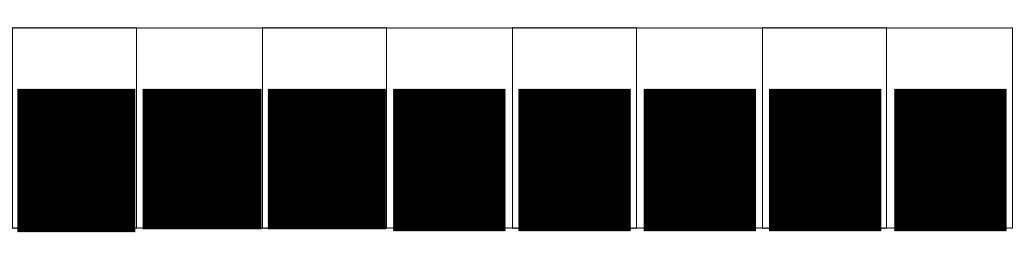
\includegraphics[width=\columnwidth]{diagrams/simple_market.pdf}

\newlength{\slotwidth}
\setlength{\slotwidth}{.103\textwidth}

\renewcommand{\arraystretch}{2}
\begin{tabular}[height=3in]{|p{\slotwidth}|p{\slotwidth}|p{\slotwidth}|p{\slotwidth}|p{\slotwidth}|p{\slotwidth}|p{\slotwidth}|p{\slotwidth}|}
\hline
Time: 0 & Time: 1 & Time: 2 & Time: 3 & Time: 4 & Time: 5 & Time: 6 & Time: 7 \\
\{(A, \$2.01)\} & \{(A, \$2.01)\} & \{(B, )\} & \{(B, )\} & \{(ISP, \$1)\} & \{(ISP, \$1)\} & \{(C, \$10)\} & \{(ISP, \$1)\} \\
\hline
\end{tabular}
\caption{Simple market sample state. User A owns the first two time slots and has an offer of \$2.01 for each. User B owns the next two slots and has not put up an offer to sell them. User C owns slot at time 6 and has posted an offer of \$10 to sell it. ISP owns remaining slots with an offer of \$1 for each.}
\label{f:simple_market}
\end{figure*}

\subsection{Simple Market Evaluation}

Simulation experiments to test whether the one-layer market has each desired property?

Measure outcome quality (vs.~SRTF or other optimal), \# of roundtrips

\begin{figure}
%\vspace{\baselineskip}
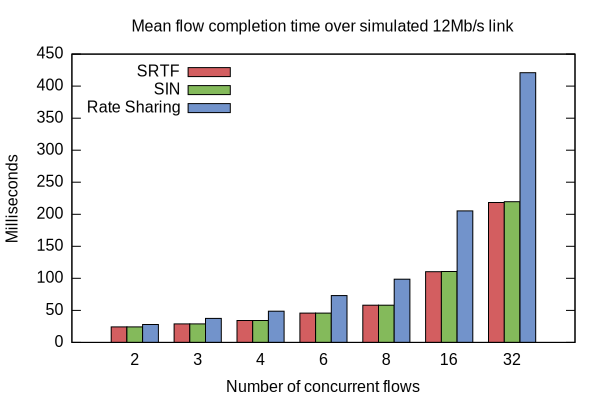
\includegraphics[width=\columnwidth]{plots/delay_over_srtf.pdf}
\caption{Flows arrive at time $uniform(0, 39)$ trying to send $uniform(1, 40)$ MTU size packets. Market can deliver 1 MTU sized packet per millisecond.}
\label{f:delay_over_srtf}
\end{figure}

We simulated the results of running a market in practice with flow completion time users that would arrive at time $t$ had a known number of packets $n$ they wanted to send.
Figure~\ref{f:delay_over_srtf} shows the result of running the simulation with 2 to 10 concurrent users, all trying to minimize their flow completion time for the cheapest cost.
We compare with a round robin scheme, which is the ideal equillibrium of mutliple TCP flows and a FIFO queued router (TODO cite).
In our simulations, there are a varying number of users with a flow start time chosen from a uniform random distribution between 0 and 9 with flow lengths chosen from a uniform random distribution between 1 and 10. We compare to the allocation of packets to times that minimizes the queued time for each flow: shortest remaining time first scheduling (TODO cite).

We find that bots in our market almost always converge on an allocation that is equivalent to the optimal shortest remaining time first schedule when there is a small number of users. Larger numbers of users are less likely to achieve a perfectly optimal solution, but the excess queuing delay over the optimal SRTF solution remains extremely low with a large number of users: less than 1\% overhead in all of our evaluations.

\subsubsection{Market Benefits}
SRTF minimizes queuing (make span?) but does not attempt to be fair to users. For example, a string of short flows will starve a long flow.
Our market recovers solutions equal or close to SRTF in terms of sum queuing delay, but it also more fairly distributes value among its users.
If a new flow arrives to a busy market, it must either wait to go after existing flows or compensate the owners of the flows it preempts. In our market, a long flow can be starved infinitely by the repeated arrival of short flows, just like SRTF, however, the owner of that flow would be compensated infintely as well to keep moving back in the order book.

TODO: it would be cool to have a graph of user utility
\subsubsection{Market Incentives}
Someone who contributes network capacity to the market would be compensated based on the prices they set.
In our current scheme, the market is acting in the interest of its users in sharing the order book and facilitating trades between users.
To incentivize the market to function efficiently, the market could potentially tax every transaction made through it. We will leave further analysis down this path for future work.

\subsubsection{User Disappointment}
Unfortunately, in this scheme it is possible that a user would have had a higher utility at the end if it refused to put offers on its slots once it successfully purchased them.
This is possible because a flow completion time user bases its offer prices on the prices the slots they would buy instead if their slots are sold, but they are not always able to purchase those replacement slots for those prices (for example if they were sold to someone else who raised the price). In an attempt to avoid this, users frequently re-price their slots, but unless their price can instantly reflect a price change, this affect is unavoidable with our current market.
%replacement slot, but if cost of that replacement slot goes up that slot can be purchased and their offer can be matched before they can re-price their offer.

This leads to a phenomena we call Disappointment, which when a user puts offers on slots it owns expecting to only increase their overall utility function in the future but instead have it reduced. User dissapointment could potentially lead to users putting higher offers or no offers at all on their slots, reducing the quality of schedules the market produces.
The User Dissapoitnment problem has parallels to the \emph{exposure problem} of auction theory \cite{milgrom00, englmaier06} because the slot prices are dependent on each other.
While user dissapointment does happen sometimes in our simulations (TODO maybe figure for this), a user normally increases their utility when they list a slot.
However, disappointment can be arbitrarily bad in the case of a hypothesized evil user: whose sole objective is to reduce the utility of another user.
\subsubsection{Evil User}
An evil user could maximally reduce the utility of a flow completion time user for the cheapest cost by buying the cheapest slot that that user has for sale, and then buying the next $m$ slots after the last packet of the flow completion time user without putting up offers for any slots. Unless the flow completion time can move earlier, this reduces the utility function of the flow completion time user by $m$. (TODO need example with reserve prices I think. Possbily diagram.)

\subsubsection{Communication overhead}

\begin{figure}
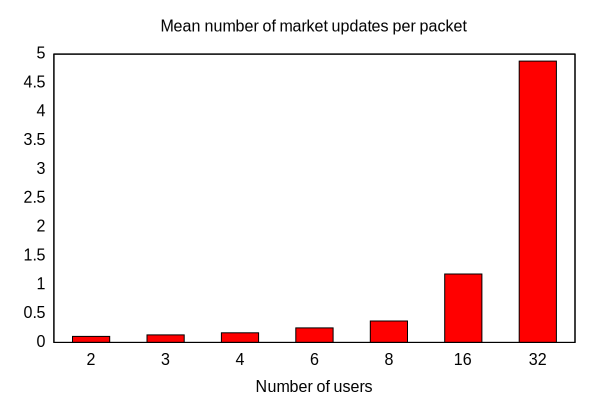
\includegraphics[width=\columnwidth]{plots/num_market_updates.pdf}
\caption{todo}
\label{f:num_market_updates}
\end{figure}

Another problem with the simple market is that it can take a long time to converge on a solution where no user wants to buy more slots. In simulation, flow completion time users buy back and forth from each other many times, making small price adjustments throughout. More contention between slots increases the number of market updates required. 
Figure~\ref{f:num_market_updates} shows the number times a user bought a set of packets on the market, or market updates, per packet sent in the simulations from in Figure~\ref{f:delay_over_srtf}.


the problems we encountered with the simple market led us to our current design:
\subsection{Multi-Layer Market Design}

Sketch of multi-layer design
